\subsection{Shared batched counter}
\label{ivl-ssec:adder}

We now show an example where IVL is inherently less costly than linearizability.
We implement an IVL batched counter, and show that its {\sc update} operation
has step complexity $O(1)$. The algorithm uses single-writer-multi-reader (SWMR) registers, \inred{which are
registers which only a single process can write to but all the processes can read from}.
In Section~\ref{ivl-ssec:lower-bound}, we prove that all \emph{linearizable} implementations
of a batched counter using SWMR registers incur step complexity $\Omega(n)$ for the {\sc update} operation.
This is in contrast with standard (non-batched) counters, which can be implemented with
a constant update time. Intuitively, the difference is that in a standard counter,
all intermediate values ``occur'' in an execution (provided that return values are
all integers and increments all add one),  and so all values allowed by IVL are also
allowed by linearizability.

% \subsubsection{IVL batched counter}
% \label{ivl-ssec:ivl-adder}

A \emph{batched counter} object supports the operations {\sc update}($v$) where $v \geq 0$, and {\sc read}().
Note that the counter's value is monotonic, as it supports only positive increments.
% We discuss the interplay between IVL and monotonicity in Section XXXX below.
The sequential specification for this object is simple: a {\sc read} operation returns the sum of all values passed to {\sc update}
operations that precede it, and $0$ if no {\sc update} operations were invoked. The {\sc update} operation returns nothing. When the
object is shared, we denote an invocation of {\sc update} by process $i$ as {\sc update}$_i$. We denote the sequential specification
of the batched counter by ${\mathcal H}$.

\begin{algorithm}
    \begin{algorithmic}[1]
        % \begin{multicols}{2}

        \State shared array $v[1 \dots n]$ initialized to $\left[0,0,\dots,0\right]$
        \Procedure{update$_i$}{$v$}
        \State $v[i] \gets v[i] + v$ \label{ivl-alg:ivl-adder:l:inc}
        \EndProcedure

        % \columnbreak

        \Procedure{read}{}
        \State $\mathit{sum} \gets 0$
        \For{$i : 1 \leq i \leq n$}
        \State $\mathit{sum} \gets \mathit{sum} + v[i]$
        \EndFor
        \State \textbf{return} $\mathit{sum}$
        \EndProcedure
    % \end{multicols}
    \end{algorithmic}
    \caption{Algorithm for process $p_i$, implementing an IVL batched counter.}
    \label{ivl-alg:ivl-adder}
\end{algorithm}

\begin{figure}[b]
    \centering
    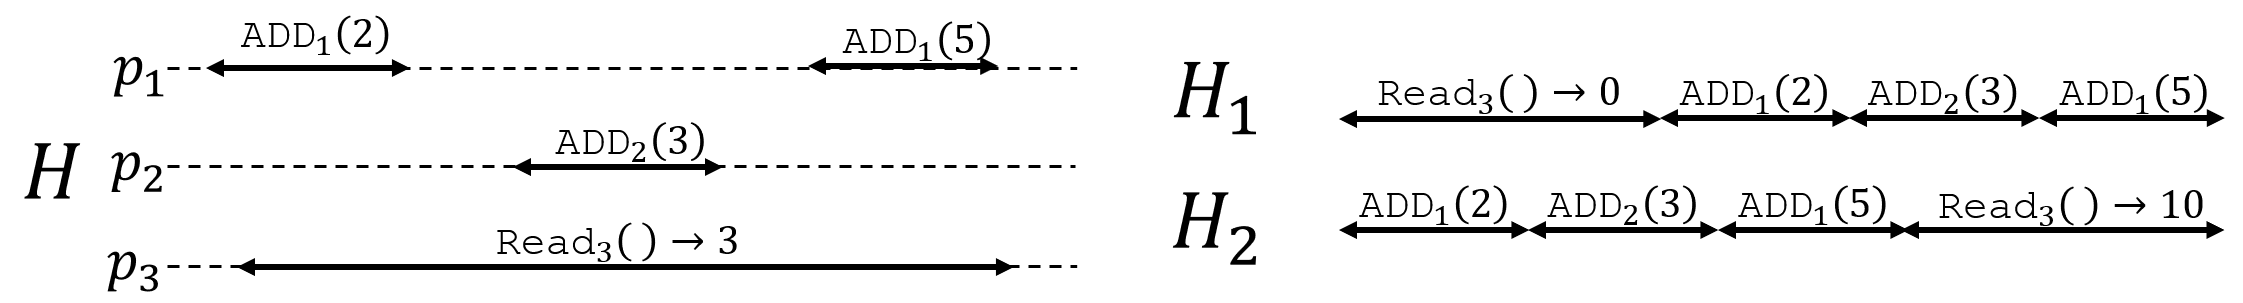
\includegraphics[width=0.7\textwidth]{graphics/ivl/adderIVL.png}
    \caption{A possible concurrent history of the IVL batched counter: $p_1$ and
    $p_2$ update their local registers, while $p_3$ reads. $p_3$ returns an intermediate
    value between the counter's state when it starts, which is $0$, and the counter's state when it completes, which is $10$.
    In $H_1$, the {\sc read} operation before all concurrent {\sc update} operations,
    and in $H_2$ it is ordered after all concurrent ones. Its return value is bounded between
    those in $H_1$, where it returns $0$, and $H_2$, where it returns $10$.}
    \label{ivl-img:adderIVL}
\end{figure}

Algorithm~\ref{ivl-alg:ivl-adder} presents an IVL implementation of a batched counter
with $n$ processes using an array $v$ of $n$ SWMR registers.
The implementation is a trivial parallelization: an {\sc update} operation increments
the process's local
register while a {\sc read} scans all registers and returns their sum. This
implementation is not linearizable because the reader does not take an atomic snapshot
of $v[1 \dots n]$. Thus, it may see a later {\sc update}
and miss an earlier one, as illustrated in Figure~\ref{ivl-img:adderIVL}.
\inred{First, note that the following observation follows from
the pseudo-code of Algorithm~\ref{ivl-alg:ivl-adder}:}
We now prove the following lemma:
\begin{lemma}
    Algorithm~\ref{ivl-alg:ivl-adder} is an IVL implementation of a batched counter.
    \label{ivl-lmma:ivl-adder}
\end{lemma}
\begin{proof}
    Let $H$ be a well-formed history of a schedule $\sigma$ of Algorithm~\ref{ivl-alg:ivl-adder},
    \inred{and let $\alpha$ be its execution}.
    We first complete $H$ be adding appropriate responses to all {\sc update} operations
    that updated $v$ (executed Line~\ref{ivl-alg:ivl-adder:l:inc}), and removing all other pending {\sc update} and {\sc read} operations.
    We denote this completed history as $H'$.

    Let $H_1$ be a linearization of $H'^?$ given by ordering {\sc update} operations by their
    return steps, and ordering {\sc read} operations after all preceding operations in $H'^?$ and before concurrent {\sc update} operations.
    {\sc read} operations assigned to the same point are ordered by their invoke steps.
    Let $H_2$ be a linearization of $H'^?$ given by ordering {\sc update} operations by their
    invocations, and ordering {\sc read} operations operations after all operations that precede them in $H'^?$ and after concurrent {\sc update} operations. 
    {\sc read} operations assigned to the same point are ordered by their invoke steps.
    Let $\alpha_i$ for $i=1,2$ be a sequential execution of a batched counter with history $\tau_\mathcal{H}(H_i)$.

    By construction, $H_1$ and $H_2$ are linearizations of $H'^?$ (as they adhere to real-time order).
    Let $R$ be some {\sc read} operation that completes
    in $H$. Let $v_{\alpha}[1 \dots n]$ be the array as read by $R$ in $\alpha$, $v_{\alpha_1}[1 \dots n]$ as read by $R$ in $\alpha_1$
    and $v_{\alpha_2}[1 \dots n]$ as read by $R$ in $\alpha_2$. To show that
    $\text{ret}(R, \tau_\mathcal{H}(H_1)) \leq \text{ret}(R, H) \leq \text{ret}(R, \tau_\mathcal{H}(H_2))$,
    we show that $v_1[j] \leq v[j] \leq v_2[j]$ for every index $1 \leq j \leq n$.

    %For any index $j$, only $p_j$ can increment $v[j]$.
    For any index $j$, $v[j]$ is incremented with non-negative values. By the construction of $H_1$, all {\sc update}
    operations that update $v[j]$ that precede $R$ in $H$ also precede it in $H_1$. Therefore, $v_{\alpha_1}[j] \leq v_{\alpha}[j]$.
    By the construction of $H_2$, all {\sc update} operations that update $v[j]$ that precede $R$ in $H$ also precede it in $H_2$.
    Furthermore, in $H_2$ all concurrent operations that have updated $v[j]$ also precede $R$. As \inred{these are} all concurrent
    {\sc update} operations that update $v[j]$, $v_{\alpha}[j] \leq v_{\alpha_2}[j]$.
    % By the construction of $H_1$, all {\sc update} operations
    % that precede $R$ in $H$ also precede it in $H_1$. Therefore $v_1[j] \leq v[j]$. Assume by contradiction that $v[j] > v_2[j]$.
    % Consider all concurrent {\sc update} operations to $R$. After all concurrent {\sc update} operations end, the value
    % of index $j$ is $v' \geq v[j] > v_2[j]$. However, by construction, $R$ is ordered after all concurrent {\sc update}
    % operations in $H_2$, therefore $v' \leq v_2[j]$. This is a contradiction, and therefore $v[j] \leq v_2[j]$.

    As all entries in the array are non-negative, it follows that $\sum_{j=1}^n v_{\alpha_1}[j] \leq \sum_{j=1}^n v_{\alpha}[j] \leq \sum_{j=1}^n v_{\alpha_2}[j]$, and
    therefore $\text{ret}(R, \tau_\mathcal{H}(H_1)) \leq \text{ret}(R, H) \leq \text{ret}(R, \tau_\mathcal{H}(H_2))$.
\end{proof}

This algorithm can efficiently implement a distributed or NUMA-friendly counter, as processes
only access their local registers \inred{for updaing values} thereby lowering the cost of incrementing the counter.\inred{Such
an implementation is highly efficient when update operations are much more frequent than read operations.}
This is of great importance, as memory latencies are often the main bottleneck in shared object emulations~\cite{mahapatra1999processor}.
As there are no waits in
either {\sc update} or {\sc read}, it follows that the algorithm is wait-free. Furthermore, the {\sc read} step complexity
is $O(n)$, and the {\sc update} step complexity is $O(1)$. Thus, we have shown the following theorem:
\begin{theorem}
    There exists a bounded wait-free IVL implementation of a batched counter using only SWMR registers, such that the step complexity of {\sc update} is $O(1)$
    and the step complexity of {\sc read} is $O(n)$.
\end{theorem}

% \subsubsection{Lower bound for linearizable batched counter object}
% \label{ivl-ssec:lower-bound}

% The incentive for using an IVL batched counter instead of a linearizable one stems
% from a lower bound on the step-complexity of a wait-free linearizable batched counter implementation from SWMR registers.
% To show the lower bound we first define the binary snapshot object.
% A \emph{snapshot object} has $n$ components written by separate processes, and allows a reader to
% capture the shared variable states of all $n$ processes instantaneously. We
% consider the \emph{binary snapshot object}, in which each state component may be either $0$ or $1$~\cite{hoepman1993binary}. The object
% supports the {\sc update}$_i$($v$) and {\sc scan} operations, where the former sets the state of component $i$
% to value a $v \in \{0,1\}$ and the latter returns all processes states instantaneously.
% It is trivial that the {\sc scan} operation must read all states, therefore its lower bound step complexity
% is $\Omega(n)$. Israeli and Shriazi~\cite{israeli1998time} show that the {\sc update} step complexity
% of any implementation of a snapshot object from SWMR registers is also $\Omega(n)$. This lower bound
% was shown to hold also for multi writer registers~\cite{attiya2006complexity}. While
% their proof was originally given for a multi value snapshot object, it holds in the binary case as well~\cite{hoepman1993binary}.

% \begin{algorithm}
%     \begin{algorithmic}[1]
%         % \begin{multicols}{2}

%         \State local variable $v_i$ \Comment{Initialized to $0$}
%         \State shared batched counter object $\mathit{BC}$
%         \Statex
%         \Procedure{update$_i$}{$v$}
%         \State \algorithmicif\ $v_i = v$\ \algorithmicthen\ \textbf{return} \label{ivl-l:skip}
%         \State $v_i \gets v$
%         \State \algorithmicif\ $v = 1$\ \algorithmicthen\ $\mathit{BC}$.{\sc update}$_i$($2^i$) \label{ivl-l:set-1}
%         \State \algorithmicif\ $v = 0$\ \algorithmicthen\ $\mathit{BC}$.{\sc update}$_i$($2^n - 2^i$) \label{ivl-l:set-0}
%         \EndProcedure
%         % \columnbreak
%         \Procedure{scan}{}
%         \State $\mathit{sum} \gets \mathit{BC}$.{\sc read}() \label{ivl-l:read} % $\mod 2^n$
%         \State $v[0 \dots n-1] \gets [0 \dots 0]$ \Comment{Initialize an array of $0$'s}
%         \For{$i : 0 \leq i \leq n-1$}
%         \State \algorithmicif\ bit $i$ is set in $\mathit{sum}$\ \algorithmicthen\ $v[i] \gets 1$ \label{ivl-l:check-set}
%         \EndFor
%         \State \textbf{return} $v[0 \dots n-1]$
%         \EndProcedure
%     % \end{multicols}
%     \end{algorithmic}
%     \caption{Algorithm for process $p_i$, solving binary snapshot with a batched counter object.}
%     \label{ivl-alg:bs-with-adder}
% \end{algorithm}

% To show a lower bound on the {\sc update} operation of wait-free linearizable batched counters,
% we show a reduction from a binary snapshot to a batched counter in
% Algorithm~\ref{ivl-alg:bs-with-adder}. It uses a local variable $v_i$ and a shared batched counter object.
% In a nutshell, the idea is to encode the value of the $i^\text{th}$ component
% of the binary snapshot using the $i^\text{th}$ least significant bit of the counter.
% When the component changes from $0$ to $1$, {\sc update}$_i$ adds $2^i$, and when it changes from $1$ to $0$,
% {\sc update}$_i$ adds $2^n - 2^i$. We now prove the following invariant:
% \begin{invariant}
%     At any point $t$ in history $H$ of a sequential execution of Algorithm~\ref{ivl-alg:bs-with-adder},
%     the sum held by the counter is $c \cdot 2^n + \sum_{i=0}^{n-1}v_i2^i$,
%     such that $v_i$ is the parameter passed to the last invocation of {\sc update}$_i$ in $H'$ before $t$ if such invocation
%     exists, and $0$ otherwise, for some integer $c \in \mathbb{N}$.
%     \label{ivl-inv:sum}
% \end{invariant}
% \begin{proof}
%     We prove the invariant by induction on the length of $H$, i.e., the number of invocations in $H$,
%     denoted $t$. As $H$ is a sequential history, each invocation is followed by a response.
%     %\par{\textbf{Base:}}
%     The base if for $t=0$, i.e., $H$ is the empty execution. In this case no updates
%     have been invoked, therefore $v_i=0$ for all $0 \leq i \leq n-1$. The sum returned by the counter
%     is $0$. Choosing $c=0$ satisfies the invariant.
%     %\par{\textbf{Induction step:}}
%     Our induction hypothesis is that the invariant holds for a history of length $t$.
%     We prove that it holds for a history of length $t+1$. The last invocation can be either a {\sc scan}, or an {\sc update}($v$)
%     by some process $p_i$. If it is a {\sc scan}, then the counter value doesn't change and the invariant
%     holds. Otherwise, it is an {\sc update}($v$). Here, we note two cases. Let $v_i$ be $p_i$'s value
%     prior to the {\sc update}($v$) invocation. If $v = v_i$, then the {\sc update} returns without altering the sum
%     and the invariant holds. Otherwise, $v \neq v_i$. We analyze two cases, $v=1$ and $v=0$. If $v=1$, then $v_i=0$.
%     The sum after the update is $c \cdot 2^n + \sum_{i=0}^{n-1}v_i2^i + 2^i=c \cdot 2^n + \sum_{i=0}^{n-1}v_i'2^i$, where
%     $v_j'=v_j$ if $j \neq i$, and $v'_i = 1$, and the invariant holds. If $v=0$, then $v_i=1$.
%     The sum after the update is $c \cdot 2^n + \sum_{i=0}^{n-1}v_i2^i + 2^n - 2^i = (c+1) \cdot 2^n + \sum_{i=0}^{n-1}v_i'2^i$,
%     where $v_j'=v_j$ if $j \neq i$, and $v'_i = 1$, and the invariant holds.
% \end{proof}

% Using the invariant, we prove the following lemma:
% \begin{lemma}
%     For any sequential history $H$, if a {\sc scan} returns $v_i$, and {\sc update}$_i$($v$) is the last update invocation in $H$
%     prior to the {\sc scan}, then $v_i = v$. If no such update exists, then $v_i=0$.
%     \label{ivl-lmma:scan-correctness}
% \end{lemma}
% \begin{proof}
%     Let $S$ be a {\sc scan} in $H'$. Consider the sum $\textit{sum}$ as read by scan $S$.
%     From Invariant~\ref{ivl-inv:sum}, the value held by the counter is $c \cdot 2^n + \sum_{i=0}^{n-1}v_i2^i$.
%     There are two cases, either there is an update invocation prior to $S$, or there isn't. If there isn't, then by
%     Invariant~\ref{ivl-inv:sum} the corresponding $v_i=0$. The process sees bit $i=0$,
%     and will return $0$. Therefore, the lemma holds.

%     Otherwise, there is a an update prior to $S$ in $H$. As the sum is equal to $c \cdot 2^n + \sum_{i=0}^{n-1}v_i2^i$,
%     by Invariant~\ref{ivl-inv:sum}, bit $i$ is equal to $1$ iff the parameter passed to the last invocation of update was $1$.
%     Therefore, the scan returns the parameter of the last update and the lemma holds.
% \end{proof}

% \begin{lemma}
%     Algorithm~\ref{ivl-alg:bs-with-adder} implements a linearizable binary snapshot using a linearizable batched counter.
%     \label{ivl-lmma:reduction}
% \end{lemma}
% \begin{proof}
%     Let $H$ be a history of Algorithm~\ref{ivl-alg:bs-with-adder}, and let $H'$
%     be $H$ where each operation is linearized at its access to the linearizable batched counter, or
%     its response if $v_i = v$ on line~\ref{ivl-l:skip}.
%     Applying Lemma~\ref{ivl-lmma:scan-correctness} to $H'$, we get $H' \in \mathcal{H}$ and therefore $H$ is linearizable.
% \end{proof}

% It follows from the algorithm that if the counter
% object is bounded wait-free then the {\sc scan} and {\sc update} operations are bounded wait-free. Therefore, the lower
% bound proved by Israeli and Shriazi~\cite{israeli1998time} holds, and the {\sc update} must take $\Omega(n)$
% steps. Other than the access to the counter in the {\sc update} operation, it takes
% $O(1)$ steps. Therefore, the access to the counter object must take $\Omega(n)$ steps. We have proven the following theorem.
% \begin{theorem}
%     For any linearizable wait-free implementation of a batched counter object with $n$ processes from SWMR registers, the step-complexity
%     of the {\sc update} operation is $\Omega(n)$.
%     \label{ivl-thm:lower-bound}
% \end{theorem}
